%%%%%%%%%%%%%%%%%%%%%%%%%%%%%%%%%%%%%%%%%%%%%%%%%
%       PRESENTAZIONE TESI 16/03/2017           %      
%%%%%%%%%%%%%%%%%%%%%%%%%%%%%%%%%%%%%%%%%%%%%%%%%

%----------------------------------------------------------------------------------------
%   PACKAGES AND THEMES
%----------------------------------------------------------------------------------------

\documentclass{beamer}

\mode<presentation> {

% The Beamer class comes with a number of default slide themes
% which change the colors and layouts of slides. Below this is a list
% of all the themes, uncomment each in turn to see what they look like.

%\usetheme{default}
%\usetheme{AnnArbor}
%\usetheme{Antibes}
%\usetheme{Bergen}
%\usetheme{Berkeley}
%\usetheme{Berlin}
%\usetheme{Boadilla}
%\usetheme{CambridgeUS}
%\usetheme{Copenhagen}
%\usetheme{Darmstadt}
%\usetheme{Dresden}
%\usetheme{Frankfurt}
%\usetheme{Goettingen}
%\usetheme{Hannover}
%\usetheme{Ilmenau}
%\usetheme{JuanLesPins}
%\usetheme{Luebeck}
\usetheme{Madrid}
%\usetheme{Malmoe}
%\usetheme{Marburg}
%\usetheme{Montpellier}
%\usetheme{PaloAlto}
%\usetheme{Pittsburgh}
%\usetheme{Rochester}
%\usetheme{Singapore}
%\usetheme{Szeged}
%\usetheme{Warsaw}

% As well as themes, the Beamer class has a number of color themes
% for any slide theme. Uncomment each of these in turn to see how it
% changes the colors of your current slide theme.

%\usecolortheme{albatross}
%\usecolortheme{beaver}
%\usecolortheme{beetle}
%\usecolortheme{crane}
%\usecolortheme{dolphin}
%\usecolortheme{dove}
%\usecolortheme{fly}
%\usecolortheme{lily}
%\usecolortheme{orchid}
%\usecolortheme{rose}
%\usecolortheme{seagull}
%\usecolortheme{seahorse}
%\usecolortheme{whale}
%\usecolortheme{wolverine}

%\setbeamertemplate{footline} % To remove the footer line in all slides uncomment this line
%\setbeamertemplate{footline}[page number] % To replace the footer line in all slides with a simple slide count uncomment this line

%\setbeamertemplate{navigation symbols}{} % To remove the navigation symbols from the bottom of all slides uncomment this line
}
\usepackage[italian]{babel}
\usepackage[utf8]{inputenc}
\usepackage{lmodern}
\usepackage{graphicx} % Allows including images
\usepackage{booktabs} % Allows the use of \toprule, \midrule and \bottomrule in tables


%----------------------------------------------------------------------------------------
%   INFO TITLE PAGE
%----------------------------------------------------------------------------------------

\title[Device-To-Device Smart Parking]{Progettazione ed implementazione di un sistema \\Smart Parking basato su comunicazione Device-To-Device}

\author{Presentata da: \\Andrea Sghedoni} % Your name
\institute[]{Alma Mater Studiorum $\cdot$ Universit\`a di Bologna \\ SCUOLA DI SCIENZE \\ Corso di Laurea Magistrale in Informatica}
\date[16/03/2017]{Sessione III \\ Anno Accademico 2015/2016} % Date, can be changed to a custom date

\begin{document}


%----------------------------------------------------------------------------------------
%   TITLE PAGE - SLIDE 1
%----------------------------------------------------------------------------------------
\begin{frame}
  \maketitle
  \textbf{Relatore:} Chiar.mo Prof. Marco Di Felice\\
  \textbf{Correlatore:} Dott. Federico Montori
\end{frame}


%----------------------------------------------------------------------------------------
%   INDEX PRESENTATION - SLIDE 2
%----------------------------------------------------------------------------------------
% [shrink=50]
\begin{frame}
  \frametitle{Indice}
  \begin{columns}
    \begin{column}{1\textwidth}
      \begin{itemize}
	\item Il parcheggio
	\item Il progetto
	\item Scenario generale
	\item Architettura software
	\item Probabilità di parcheggio
	\item Tecnologie
	\item Screenshot
	\item Simulazione e Modellazione
	\item Risultati
	\item Conclusioni
      \end{itemize}
    \end{column}
  \end{columns}
\end{frame}


%----------------------------------------------------------------------------------------
%   PROBLEMA DEL PARCHEGGIO - SLIDE 3
%----------------------------------------------------------------------------------------
\begin{frame}
  \frametitle{Il parcheggio}
  \begin{itemize}
    \item Il continuo processo di urbanizzazione ha portato sovraffollamento di autoveicoli nelle città metropolitane
    \item Più del 30\% della congestione del traffico è causata da utenti in cerca di parcheggio
    \item Parcheggi on-street
    \item Conseguenze negative:
    \begin{itemize}
      \item perdita di tempo e denaro
      \item inquinamento ambientale (CO\ped{2})
      \item peggioramento della qualità di vita
    \end{itemize}
  \end{itemize}
\end{frame}


%----------------------------------------------------------------------------------------
%   IL PROGETTO - SLIDE 4
%----------------------------------------------------------------------------------------
\begin{frame}
  \frametitle{Il progetto}
  \begin{itemize}
    \item Sistema di Smart Parking in grado di favorire l'attività di parcheggio all'utente 
    \item Miglior gestione dei parcheggi 
    \item \textit{Crowdsensing} e condivisione dei dati con la comunità
    \item Determinare la probabilità di parcheggio nelle zone limitrofe alla posizione corrente
    \item Assenza di strutture centralizzate
    \item Disseminazione dell'informazione Device-To-Device (D2D) completamente distribuita
    \item Meccanismo di spreading automatico e trasparente all'utente
  \end{itemize}
\end{frame}


%----------------------------------------------------------------------------------------
%   SCENARIO GENERALE E RUOLI UTENTE - SLIDE 5
%----------------------------------------------------------------------------------------
\begin{frame}
  \frametitle{Scenario generale}
  \begin{columns}
    \begin{column}{0.6\textwidth}
      \begin{itemize}
	\item Città metropolitana
	\item Alta dinamicità
	\item Griglia logica suddivide la città
	\item Per ogni cella si stima la probabilità di parcheggio
	\item Ruoli dei device durante la sincronizzazione:
	\begin{itemize}
	  \item Access Point
	  \item client
	\end{itemize}
      \end{itemize}
    \end{column}

    \begin{column}{0.4\textwidth}
      \begin{figure}
	\raggedleft
	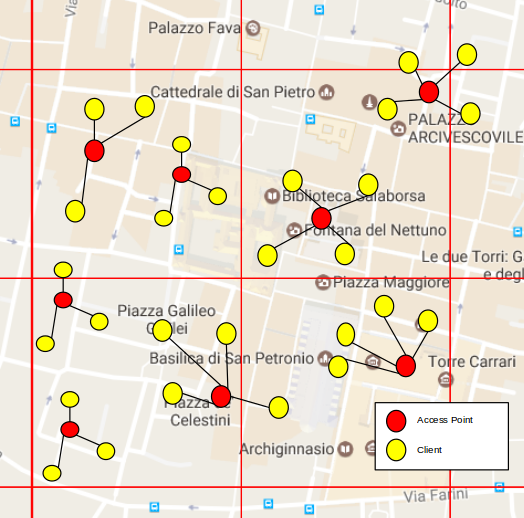
\includegraphics[width=\columnwidth]{img/arch_general.png}
      \end{figure}
    \end{column}
  \end{columns}
\end{frame}


%----------------------------------------------------------------------------------------
%   ARCH. SOFTWARE - SLIDE 6
%----------------------------------------------------------------------------------------
\begin{frame}
  \frametitle{Architettura software}
  \begin{columns}
    \begin{column}{0.5\textwidth}
      \begin{enumerate}
	\item Componente di \textit{\textbf{Activity Recognition}} rileva eventi di parcheggio e rilascio
	\item Il \textit{\textbf{Local DB}} salva informazioni sui parcheggi e le ultme sincronizzazioni efettuate
	\item Il \textit{\textbf{Controller}} funge da interfaccia verso il database
	\item Il \textit{\textbf{Dissemination Service}} sincronizza le informazioni in modalità D2D con altri peer nei paraggi
      \end{enumerate}
    \end{column}

    \begin{column}{0.5\textwidth}
      \begin{figure}
	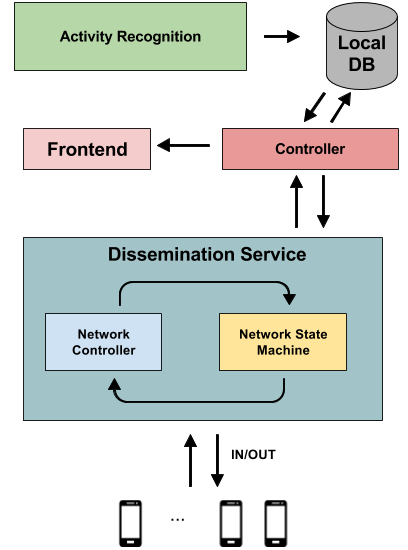
\includegraphics[scale=0.30]{img/arch_soft2.png}
      \end{figure}
    \end{column}
  \end{columns}
\end{frame}


%----------------------------------------------------------------------------------------
%   PROBABILITA - SLIDE 7
%----------------------------------------------------------------------------------------
\begin{frame}
  \frametitle{Probabilità di parcheggio}

  \begin{itemize}
    \item Sincronizzazione sugli eventi parcheggio/rilascio della cella \textit{i}
    \item Eventi parcheggio $E\ped{i}\ap{p}$ e rilascio $E\ped{i}\ap{r}$
    \item Slot totali $N\ped{i}\ap{t}$ noto a priori
    \item Slot occupati:
    \\
    {\centering $N\ped{i}\ap{o} = E\ped{i}\ap{p} - E\ped{i}\ap{r}$\par}
    \vspace{2mm}
    \item Tasso di occupazione:
    \\
    {\centering $p\ped{i}\ap{o} = \frac{N\ped{i}\ap{o}}{N\ped{i}\ap{t}}$\par}
    \vspace{2mm}
    \item Probabilità di trovare parcheggio:
    \\
    \vspace{4mm}
    \centering \framebox{$p\ped{i}\ap{f} = 1 - p\ped{i}\ap{o}$}
  \end{itemize}
\end{frame}


%----------------------------------------------------------------------------------------
%   TECNOLOGIE - SLIDE 8
%----------------------------------------------------------------------------------------
\begin{frame}
  \frametitle{Tecnologie utilizzate}
  \begin{columns}
   \begin{column}{0.5\textwidth}
    \begin{itemize}
      \item SO \textit{\textbf{Android 4.0}} e superiori\vspace{5mm}
      \item \textit{\textbf{WiFi Direct}}
      \begin{itemize}\vspace{1mm}
      \item \textit{\textbf{Peer-To-Peer (P2P) Group}}\vspace{1mm}
      \item \textit{\textbf{Bonjour beacon}}\vspace{1mm}
      \item serialized \textit{\textbf{Socket}}\vspace{5mm}
      \end{itemize}
      \item \textit{\textbf{SQLite}}\vspace{5mm}
    \end{itemize}
   \end{column}
   \begin{column}{0.5\textwidth}
    \begin{figure}
      
\includegraphics[scale=0.08]{img/android.png}
    \end{figure}
     \begin{figure}
       
\includegraphics[scale=1.9]{img/wifidirect.png}
     \end{figure}
     \begin{figure}
       
\includegraphics[scale=0.14]{img/sqlite.png}
     \end{figure}
    \end{column}
  \end{columns}
\end{frame}


%----------------------------------------------------------------------------------------
%   SCREENSHOT 1 - SLIDE 9
%----------------------------------------------------------------------------------------
\begin{frame}
  \frametitle{Screenshot 1}
  \begin{columns}
    \begin{column}{0.25\textwidth}
      \begin{figure}
      \raggedleft
      \setlength{\fboxsep}{0pt}
      \setlength{\fboxrule}{0.1pt}
      \fcolorbox{blue}{blue}{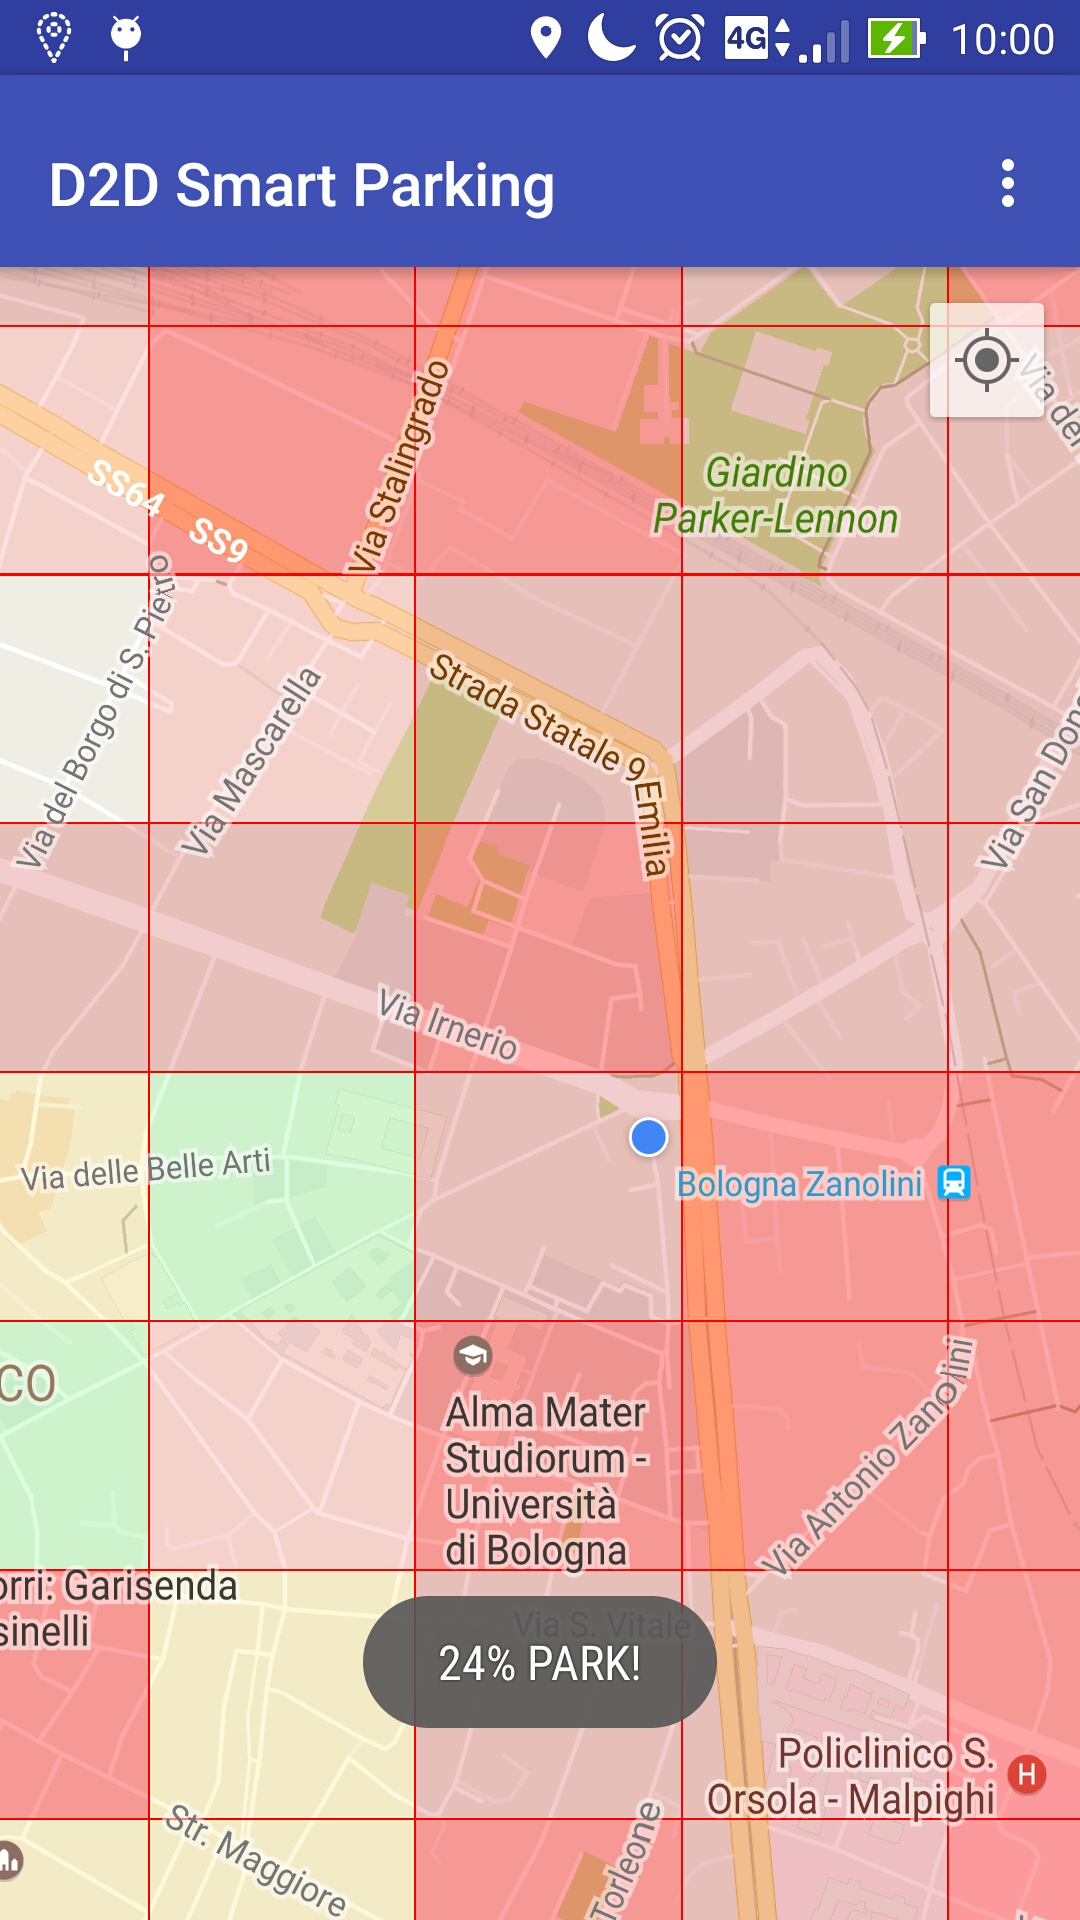
\includegraphics[width=\columnwidth]{img/screenshot/map2.jpg}}
      \end{figure}
    \end{column}
    \begin{column}{0.25\textwidth}
      \begin{figure}
      \raggedleft
      \setlength{\fboxsep}{0pt}
      \setlength{\fboxrule}{0.1pt}
      \fcolorbox{blue}{blue}{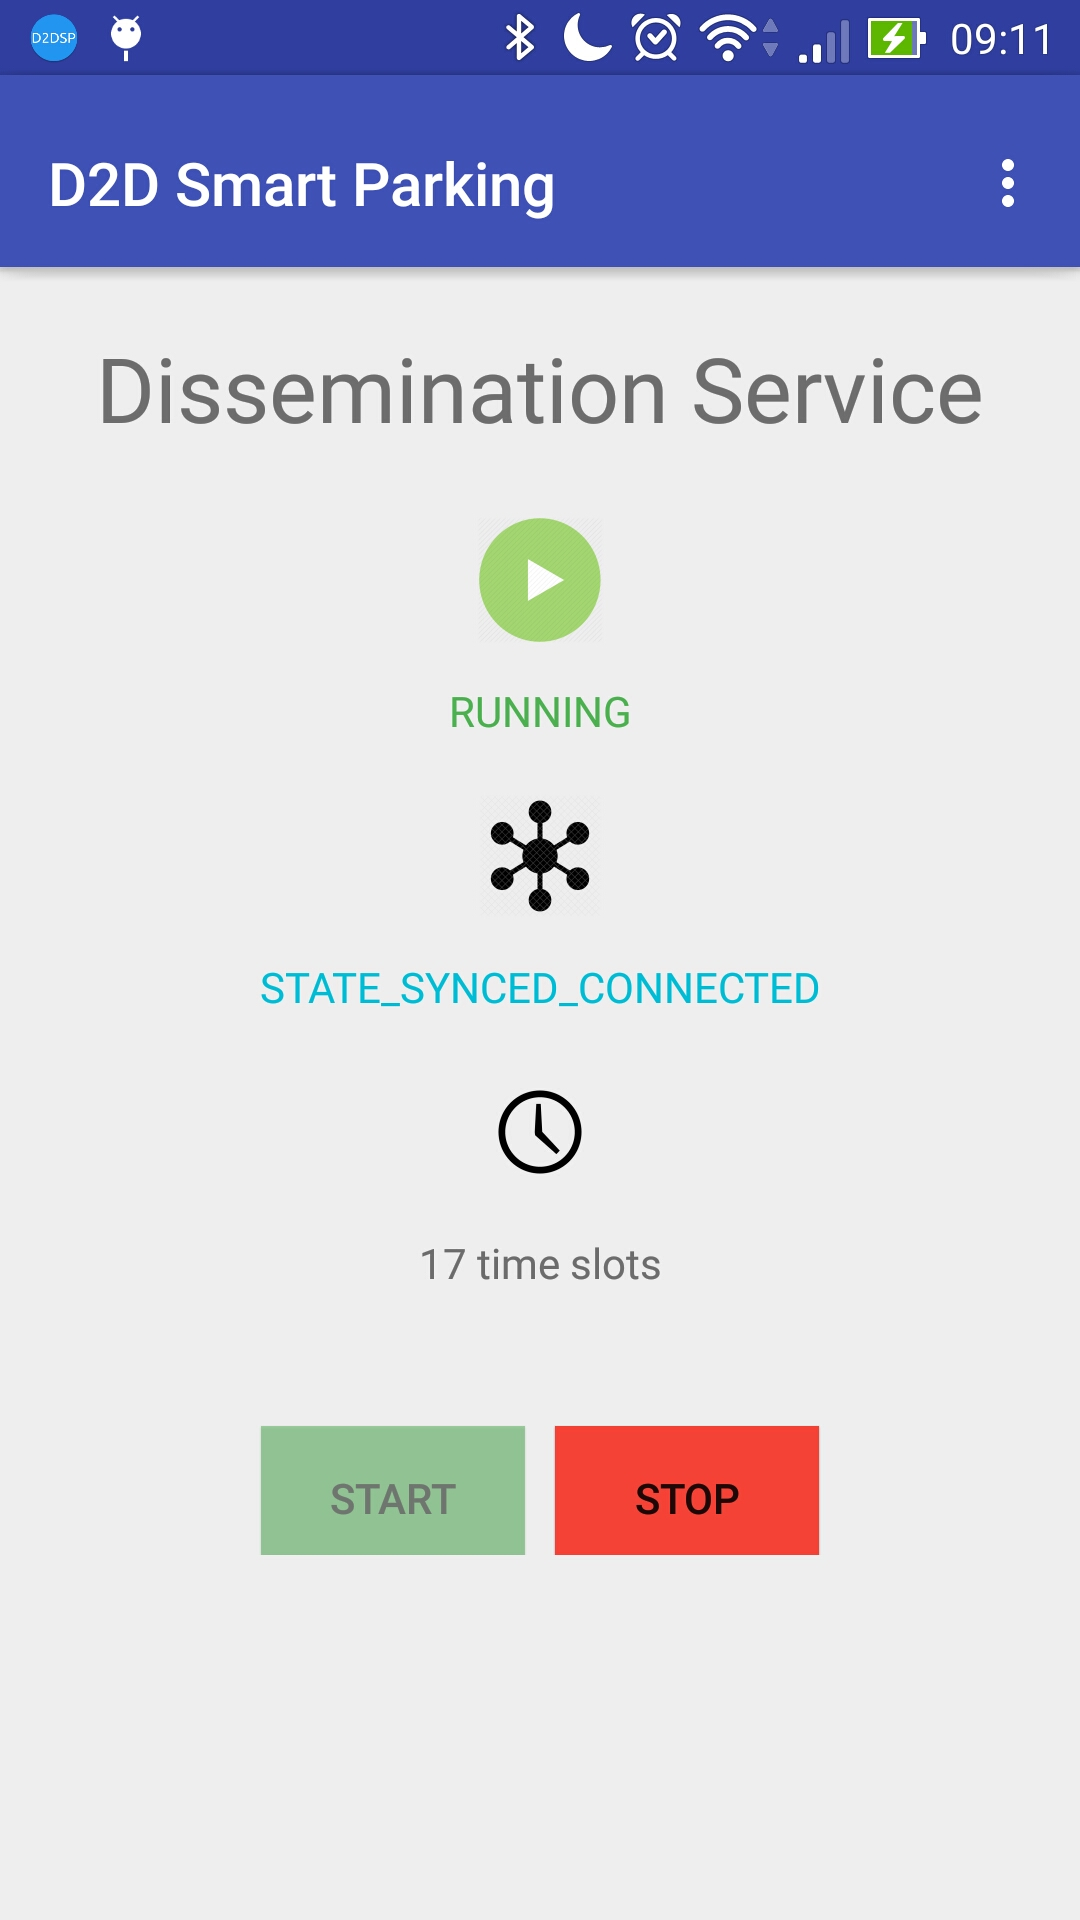
\includegraphics[width=\columnwidth]{img/screenshot/state_synced_connected.jpg}}
      \end{figure}
    \end{column}
    \begin{column}{0.25\textwidth}
      \begin{figure}
      \raggedleft
      \setlength{\fboxsep}{0pt}
      \setlength{\fboxrule}{0.1pt}
      \fcolorbox{blue}{blue}{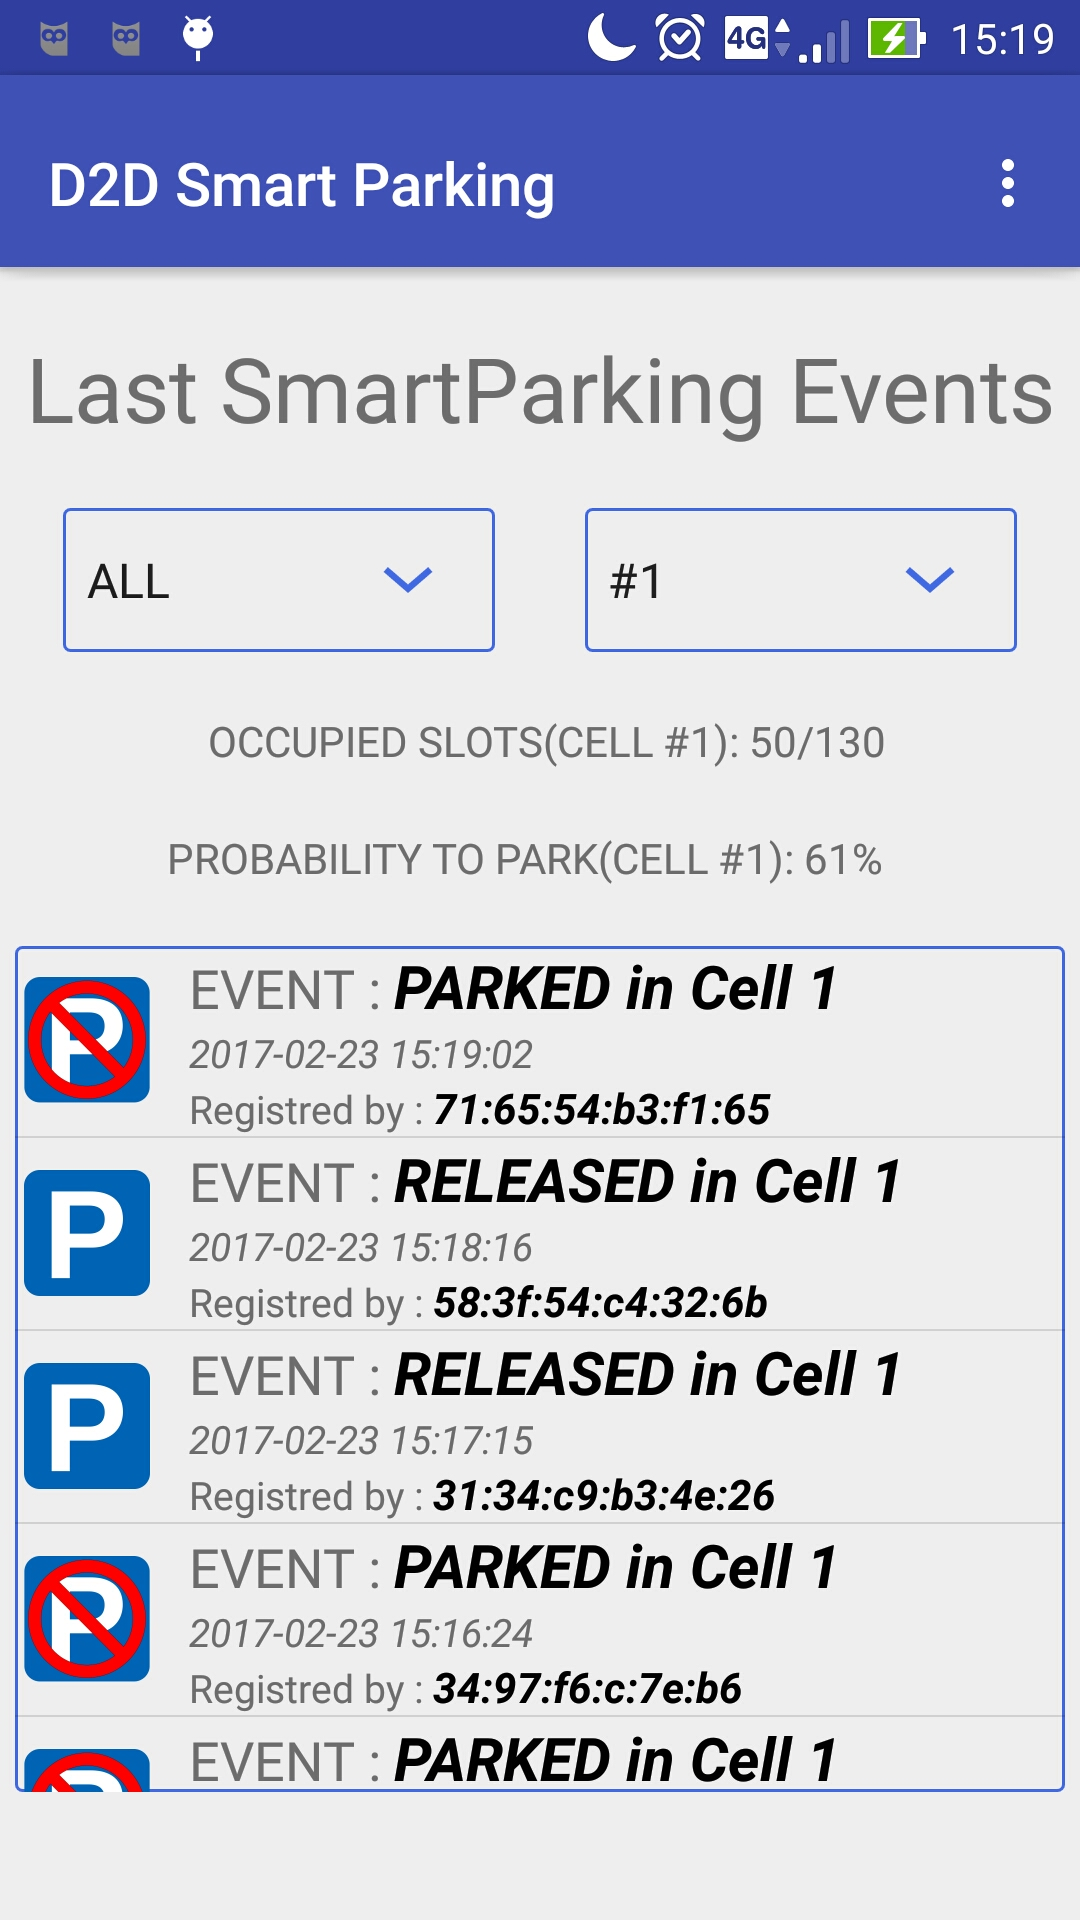
\includegraphics[width=\columnwidth]{img/screenshot/park_event_list.jpg}}
      \end{figure}
    \end{column}
    \begin{column}{0.25\textwidth}
      \begin{figure}
      \raggedleft
      \setlength{\fboxsep}{0pt}
      \setlength{\fboxrule}{0.1pt}
      \fcolorbox{blue}{blue}{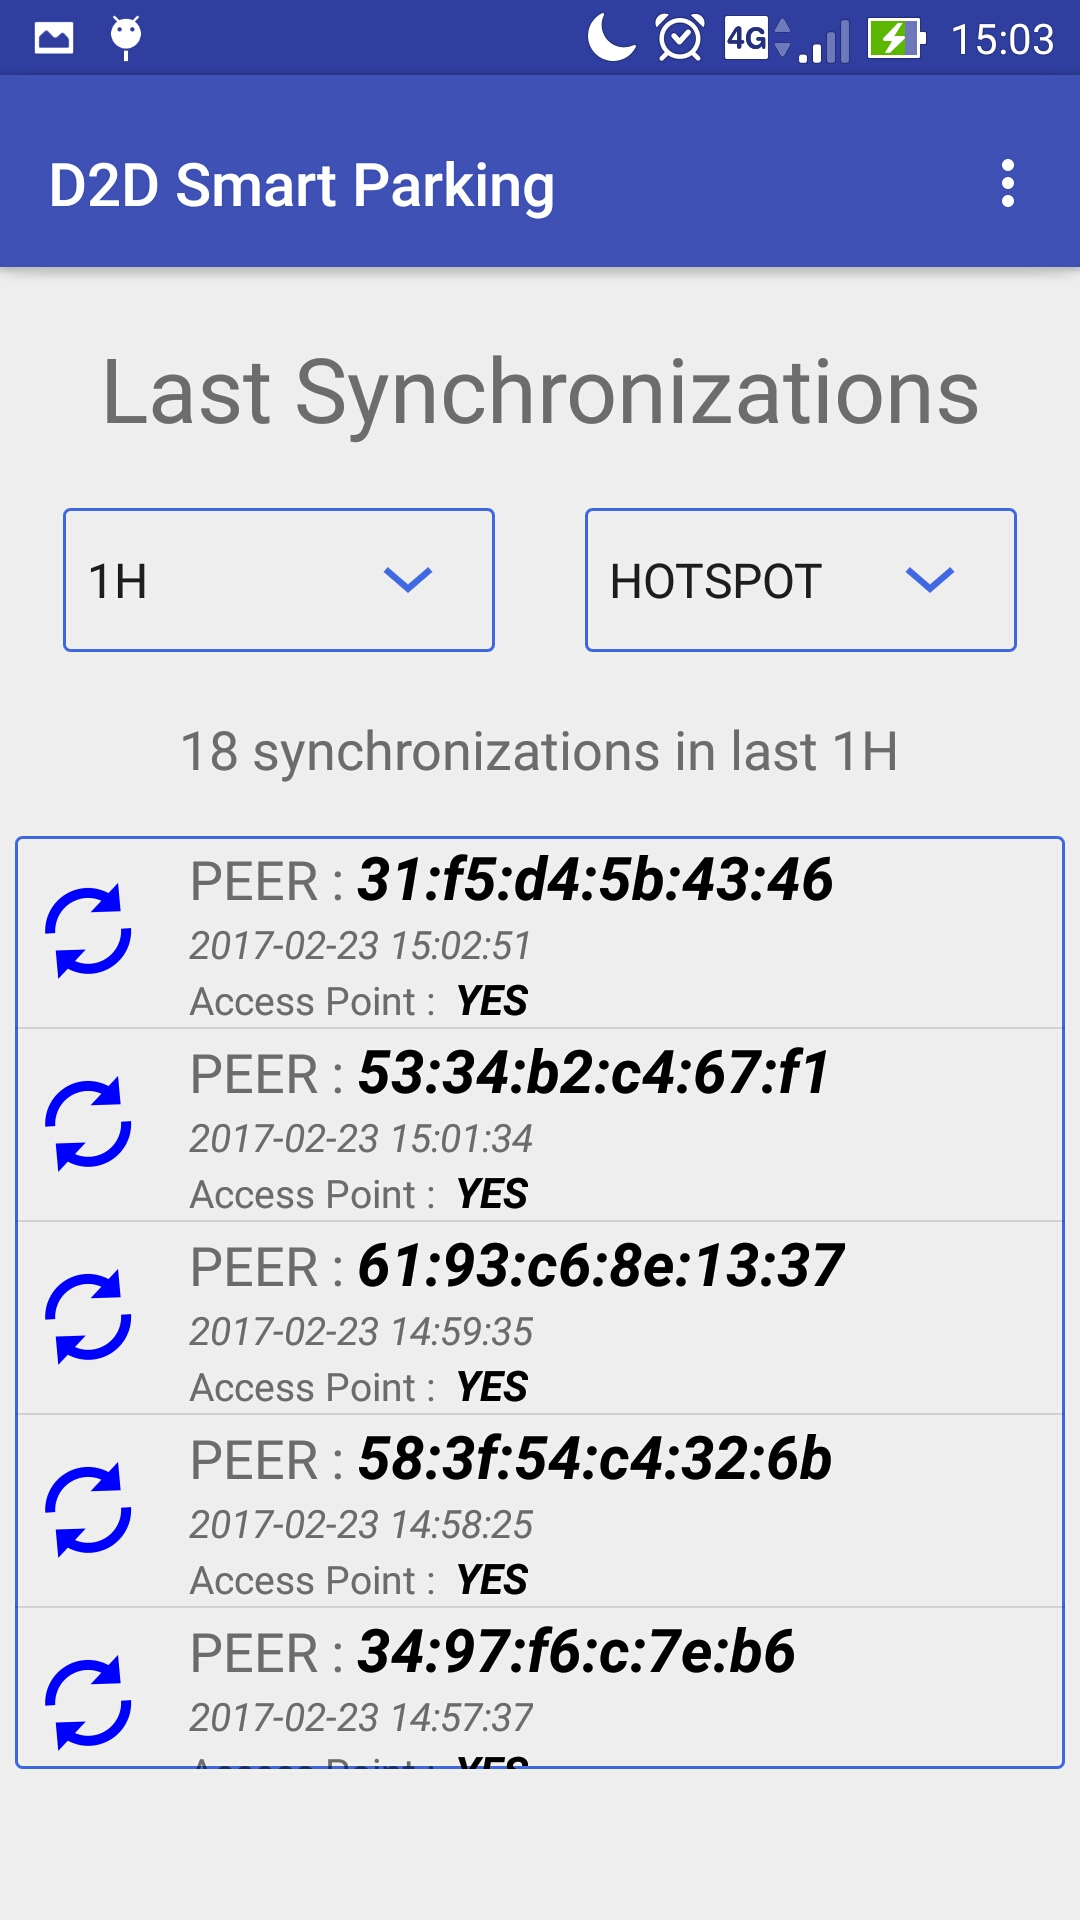
\includegraphics[width=\columnwidth]{img/screenshot/last_sync.jpg}}
      \end{figure}
    \end{column}
  \end{columns}
\end{frame}


%----------------------------------------------------------------------------------------
%   SIMULAZIONE - SLIDE 10
%----------------------------------------------------------------------------------------
\begin{frame}
  \frametitle{Simulazione e Modellazione}
  \begin{columns}
    \begin{column}{0.65\textwidth}
      \begin{itemize}
	\item OMNeT++, Veins, SUMO
	\item Zona nord-est di Bologna 1.5km x 2.5km
	\item Verificare l’efficacia del processo di spreading
	\item circa 3000 veicoli in 1800 simsec
	\item Modulo \textit{SmartParking} per modellazione logica
	\item Tecnologie considerate: 
	  \begin{itemize}
	    \item V2V \textit{802.11p}
	    \item D2D \textit{WiFi Direct} 
	    \item \textit{Bluetooth}
	  \end{itemize}
      \end{itemize}
    \end{column}

    \begin{column}{0.35\textwidth}
      \begin{figure}
      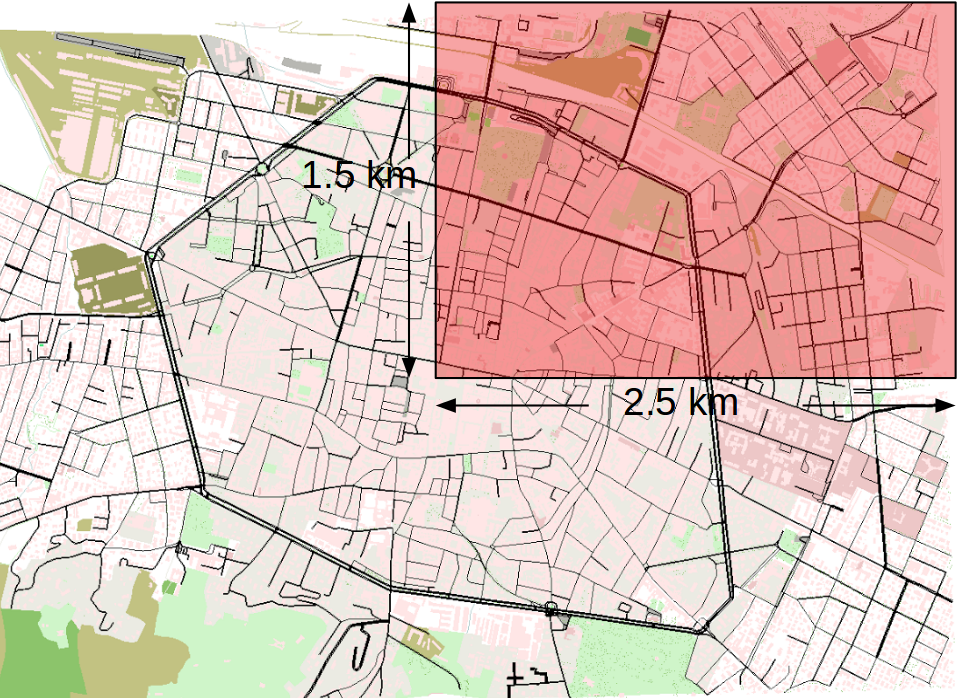
\includegraphics[width=\columnwidth]{img/sumo-bolo2.png}
      \end{figure}
    \end{column}
  \end{columns}
\end{frame}


%----------------------------------------------------------------------------------------
%   RISULTATI 1 - SLIDE 11
%----------------------------------------------------------------------------------------
\begin{frame}
  \frametitle{Risultati (1)}
  \begin{itemize}
    \item convergenza sulla conoscenza della cella corrente e dello scenario generale
  \end{itemize}
  \begin{columns}
    \begin{column}{0.45\textwidth}
      \begin{figure}
	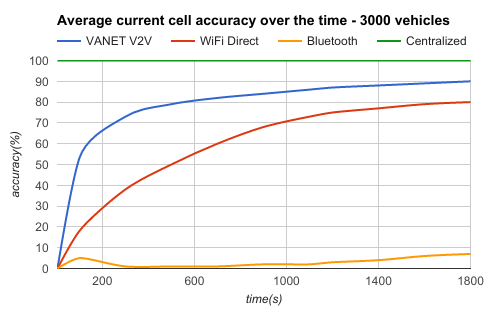
\includegraphics[width=\columnwidth]{img/graphics/local_accuracy.png}
      \end{figure}
      
    \end{column}
    \begin{column}{0.45\textwidth}
      \begin{figure}
	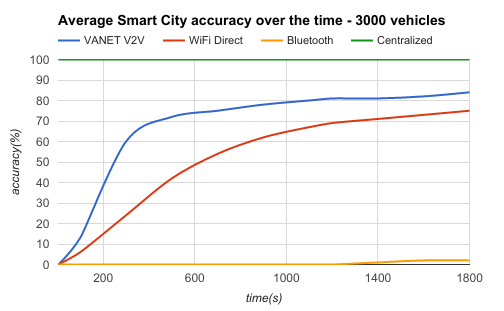
\includegraphics[width=\columnwidth]{img/graphics/global_accuracy.png}
      \end{figure}
    \end{column}
  \end{columns}
\end{frame}


%----------------------------------------------------------------------------------------
%   RISULTATI 2 - SLIDE 12
%----------------------------------------------------------------------------------------
\begin{frame}[shrink=40]
  \frametitle{Risultati (2)}
  \begin{columns}
    \begin{column}{0.45\textwidth}
      \vspace{20mm}
      \begin{figure}
      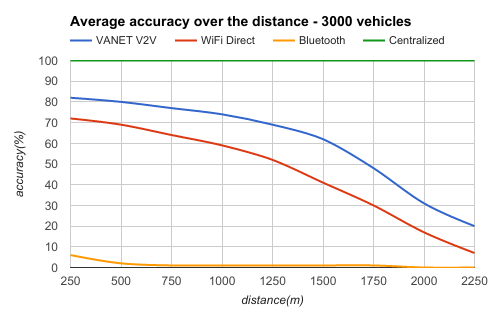
\includegraphics[width=\columnwidth]{img/graphics/distance.png}
      \end{figure}
      \begin{itemize}
	\item  L'accuratezza media decresce all'aumentare della distanza dalla posizione corrente
	\item  L'accuratezza migliore nel raggio di 500m della posizione corrente (sincronizzazioni su cella corrente e adiacenti)
      \end{itemize}
    \end{column}
    \begin{column}{0.45\textwidth}
      \vspace{10mm}
      \begin{figure}
      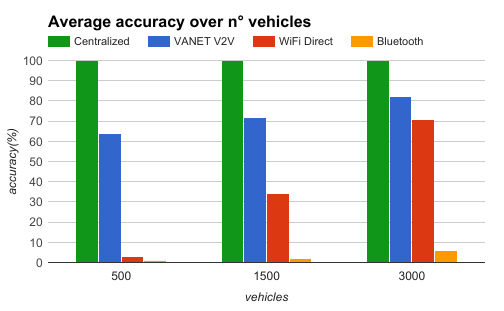
\includegraphics[width=\columnwidth]{img/graphics/n_car.png}
      \end{figure}
      \begin{itemize}
	\item  Tasso di partecipazione determinante per la tecnologia D2D \textit{WiFi Direct}
      \end{itemize}
    \end{column}
  \end{columns}
\end{frame}


%----------------------------------------------------------------------------------------
%   CONCLUSIONI - SLIDE 13
%----------------------------------------------------------------------------------------
\begin{frame}
\frametitle{Conclusioni}
  \begin{itemize}
    \item Sistema di Smart Parking con l'obiettivo di ottimizzare i parcheggi e favorire la viabilità generale
    \item L'utente ottiene in tempo reale la situazione parcheggi nei paraggi
    \item Tecnologia \textit{WiFi Direct} con alto tasso di partecipazione può ottenere buoni risultati confrontandosi con tecnologie più costose e complesse (\textit{V2V 802.11p})
    \item Sviluppi futuri: 
      \begin{itemize}
	\item risparmio energetico sulle attività D2D
	\item guidare l'utente verso le zone meno congestionate in base alla destinazione
	\item prevedere un servizio light centralizzato
	\item individuare e favorire le sincronizzazioni che permettano di aumentare il processo di spreading
      \end{itemize}
  \end{itemize}
\end{frame}


%----------------------------------------------------------------------------------------
%   GRAZIE PER ATTENZIONE - SLIDE 14
%----------------------------------------------------------------------------------------
\begin{frame}
\Huge{\centerline{Grazie per l'attenzione!}}
\end{frame}


%----------------------------------------------------------------------------------------
%   FINISH
%----------------------------------------------------------------------------------------
\end{document}



%----------------------------------------------------------------------------------------
%   CROWDSENSING PRESENTATION SLIDE 4
%----------------------------------------------------------------------------------------
% \begin{frame}
% \frametitle{Il Crowdsensing}
% \begin{itemize}
%   \item Condivisione di dati con la collettività
%   \item Intelligenza condivisa
%   \item Il singolo contribuisce al benessere collettivo
% \end{itemize}
% \end{frame}